\documentclass[12pt,a4paper,oneside]{report}
\usepackage[utf8]{inputenc}
\usepackage[T1]{fontenc}
\usepackage{amsmath, amssymb, amsfonts}
\usepackage{graphicx}
\usepackage{hyperref}
\usepackage{geometry}
\usepackage{booktabs}
\usepackage{titlesec}
\usepackage{listings}
\usepackage{xcolor}
\usepackage{caption}
\usepackage{subcaption}
\usepackage{tikz}
\usetikzlibrary{shapes.geometric, arrows}

\geometry{margin=1in}
\hypersetup{colorlinks=true, linkcolor=blue, urlcolor=cyan}

\definecolor{codegray}{rgb}{0.5,0.5,0.5}
\definecolor{codepurple}{rgb}{0.58,0,0.82}
\definecolor{backcolour}{rgb}{0.95,0.95,0.92}

\lstdefinestyle{mystyle}{
    backgroundcolor=\color{backcolour},   
    commentstyle=\color{green!60!black},
    keywordstyle=\color{magenta},
    numberstyle=\tiny\color{codegray},
    stringstyle=\color{codepurple},
    basicstyle=\ttfamily\footnotesize,
    breakatwhitespace=false,         
    breaklines=true,                 
    captionpos=b,                    
    keepspaces=true,                 
    numbers=left,                    
    numbersep=5pt,                  
    showspaces=false,                
    showstringspaces=false,
    showtabs=false,                  
    tabsize=2
}
\lstset{style=mystyle}

\title{\textbf{NS-CausalKT: Neural-Symbolic Causal Knowledge Tracing for Intelligent Tutoring Systems}}
\author{Your Name}
\date{May 2026}

\begin{document}

\maketitle

\begin{abstract}
Knowledge Tracing (KT) is a critical task in personalized education, aimed at modeling student knowledge states over time. While deep learning models have significantly improved predictive performance, they lack causal interpretability and symbolic grounding. This report presents NS-CausalKT, a novel Neuro-Symbolic Causal Knowledge Tracing framework. Our model integrates a Transformer-based neural encoder with a Symbolic Concept Layer for prerequisite enforcement and a Causal SCM Layer for intervention simulation. Experimental results on the ASSISTments 2009 dataset demonstrate that NS-CausalKT achieves a competitive AUC of 0.8137 while providing actionable causal insights. We also introduce an "Agentic Grader" prototype that leverages multimodal LLMs for automated feedback.
\end{abstract}

\newpage
\tableofcontents
\newpage
\listoffigures
\newpage
\listoftables

\newpage
\chapter{Introduction}

\section{Background}
The rapid growth of online learning platforms and Intelligent Tutoring Systems (ITS) has generated massive amounts of educational data. At the heart of these systems is the task of Knowledge Tracing (KT), which involves tracking a student's mastery of specific concepts or skills over time based on their sequence of interactions with the system. Accurately modeling a student's knowledge is essential for personalizing learning paths, recommending the next best content, and providing timely interventions.

\section{Motivation}
Despite the success of deep learning in KT, most state-of-the-art models operate as "black boxes." While models like Deep Knowledge Tracing (DKT) and Attentive Knowledge Tracing (AKT) can predict with high accuracy whether a student will answer the next question correctly, they cannot explain the underlying reason for failure. In educational contexts, understanding "why" a student failed is often more important than knowing "that" they will fail. Specifically, existing models lack:
\begin{itemize}
    \item \textbf{Causal Interpretability}: They cannot distinguish between mere correlation and actual causation in skill mastery.
    \item \textbf{Symbolic Grounding}: They often ignore the structured domain knowledge, such as prerequisite relationships between math concepts.
    \item \textbf{Intervention Support}: They cannot simulate the effect of teaching a specific concept before another (counterfactual reasoning).
\end{itemize}

\section{Problem Statement}
The core problem addressed in this project is the lack of causal transparency and logical consistency in current Knowledge Tracing architectures. We aim to develop a model that not only predicts student performance but also identifies the root causes of learning gaps and allows for "what-if" simulations through causal interventions.

\section{Objectives}
The primary objectives of this project are:
\begin{enumerate}
    \item To design and implement **NS-CausalKT**, a Neuro-Symbolic Causal Knowledge Tracing framework.
    \item To integrate symbolic prerequisite rules into a neural transformer architecture using Logic Tensor Networks (LTN).
    \item To implement a Structural Causal Model (SCM) capable of performing do-calculus interventions.
    \item To develop an **Agentic UI** prototype that uses multimodal AI for automated, diagnostic grading.
\end{enumerate}

\section{Project Scope}
This project covers the full lifecycle of a machine learning system, from data preprocessing of the ASSISTments 2009 dataset to the deployment of a full-stack web application. The scope includes model architecture design, training optimization, causal metric evaluation, and frontend development for data visualization.

\chapter{Literature Review}

\section{Evolution of Knowledge Tracing}
Knowledge Tracing has been a core research topic in educational technology for over three decades. The field has transitioned from simple probabilistic models to complex deep learning architectures.

\subsection{Bayesian Knowledge Tracing (BKT)}
Introduced by Corbett and Anderson in 1994, BKT is a Hidden Markov Model (HMM) where each skill is modeled as a binary latent variable (known or unknown). BKT uses four parameters: $P(L_0)$ (initial knowledge), $P(T)$ (learning rate), $P(G)$ (guess), and $P(S)$ (slip). While BKT is highly interpretable, it struggles with modeling multiple skills simultaneously and ignores the order of interactions.

\subsection{Deep Knowledge Tracing (DKT)}
In 2015, Piech et al. introduced DKT, the first model to use Recurrent Neural Networks (LSTMs) for KT. DKT treats the whole interaction history as a single sequence, allowing it to capture complex learning patterns that BKT misses. However, DKT is criticized for being a "black box" and for having "noisy" latent states that sometimes violate logical prerequisites.

\section{Attention-Based Models}
To address the limitations of LSTMs in handling long-term dependencies, researchers introduced Attention mechanisms to KT.

\subsection{SAKT and AKT}
SAKT (Self-Attentive Knowledge Tracing) and AKT (Attentive Knowledge Tracing) use the Transformer architecture. AKT, in particular, introduced context-aware embeddings that consider the time elapsed between interactions. These models significantly improved AUC scores on benchmarks like ASSISTments 2009 but remained purely correlational.

\section{Causal Inference in Education}
Causal inference, pioneered by Judea Pearl, provides a mathematical framework for understanding cause-and-effect through the Structural Causal Model (SCM). In education, causality is vital for identifying whether a student's failure in Algebra is \textit{caused} by a gap in Fractions or just correlated with it.

\section{Neuro-Symbolic AI}
Neuro-symbolic systems combine the robust learning capabilities of neural networks with the hard logical constraints of symbolic reasoning. Logic Tensor Networks (LTN) are a prominent technique in this area, allowing logical formulas to be used as differentiable terms in a loss function. This project leverages LTNs to ensure that the student's predicted knowledge state respects the curriculum's prerequisite graph.

\chapter{Methodology}

\section{System Architecture}
The NS-CausalKT model is designed as a three-layered architecture. Each layer addresses a specific aspect of the learning process: neural sequence modeling, symbolic constraint enforcement, and causal intervention.

\subsection{Neural Student Model (NSM)}
The NSM uses a 2-layer Transformer encoder with multi-head attention. For each student interaction $(q_t, a_t)$, we create an embedding $e_t$:
\begin{equation}
    e_t = \text{Embed}(q_t) \oplus \text{Embed}(a_t) \oplus \text{Embed}(c_t) \oplus \Delta t_t
\end{equation}
The Transformer output $H$ is then refined through a GRU to capture temporal dynamics like the spacing effect (forgetting curves).

\subsection{Symbolic Concept Layer (SCL)}
The SCL ensures that the latent knowledge state $\mu_t$ follows the rules of the domain. We define a Directed Acyclic Graph (DAG) $G$ representing concept prerequisites. We use **Logic Tensor Networks (LTN)** to define soft rules. For example, the "Prerequisite Necessity" rule states:
\begin{equation}
    \forall s, t: \text{masters}(s, c_i, t) \implies \text{masters}(s, c_j, t) \text{ if } (c_j \to c_i) \in E
\end{equation}
This rule is enforced using the Łukasiewicz t-norm, making the logic differentiable and suitable for gradient-based training.

\subsection{Causal SCM Layer (CSL)}
The CSL implements a Structural Causal Model (SCM). The Average Causal Effect (ACE) of a concept $c_j$ on the student's performance $a_{t+1}$ is computed using Pearl's do-calculus:
\begin{equation}
    \text{ACE}(c_j \to a_{t+1}) = E[a_{t+1} | do(c_j=1)] - E[a_{t+1} | do(c_j=0)]
\end{equation}
By computing ACE for all prerequisite concepts, we can identify the "Root Cause" of a student's failure.

\section{Loss Functions}
The model is trained end-to-end using a joint objective function $L_{total}$:
\begin{equation}
    L_{total} = L_{pred} + \lambda_1 L_{sym} + \lambda_2 L_{causal} + \lambda_3 L_{smooth}
\end{equation}
Where:
\begin{itemize}
    \item $L_{pred}$ is the Binary Cross-Entropy loss for performance prediction.
    \item $L_{sym}$ ensures consistency with the prerequisite graph.
    \item $L_{causal}$ regularizes the mastery state based on causal constraints.
    \item $L_{smooth}$ penalizes sudden, unrealistic jumps in knowledge mastery.
\end{itemize}

\section{Data Preprocessing}
The ASSISTments 2009 dataset was preprocessed to remove noise and ensure consistency.
\begin{itemize}
    \item \textbf{Sequence Length}: Sequences were truncated or padded to a fixed length of 200 interactions.
    \item \textbf{Concept Mapping}: Each problem was mapped to a unique skill ID.
    \item \textbf{Splitting}: A student-level 80/20 split was used for training and validation to prevent data leakage.
\end{itemize}

\chapter{Implementation \& Prototype}

\section{Technology Stack}
The system is built as a full-stack web application. The core logic is implemented in Python, while the user interface is developed using modern web technologies.

\subsection{Backend}
The backend is a **Flask** application that provides several API endpoints:
\begin{itemize}
    \item \texttt{/api/dashboard}: Returns real-time metrics (AUC, ACC) and training logs.
    \item \texttt{/api/causal}: Provides data for the causal DAG and ACE rankings.
    \item \texttt{/api/analyze}: The core endpoint for the "Agentic Grader," which processes images using GPT-4o Mini.
\end{itemize}

\subsection{Frontend}
The frontend is built using **HTML5, Vanilla CSS, and JavaScript**. We avoided heavy frameworks like React to ensure maximum performance and maintainability. Key components include:
\begin{itemize}
    \item **Interactive Charts**: Using CSS-based bars and custom SVG visualizations for the concept mastery timeline.
    \item **Live Document Viewer**: A PDF/Image viewer that overlays "bounding boxes" detected by the AI.
\end{itemize}

\section{Agentic Grading System}
The "Agentic" part of the project leverages the multimodal capabilities of **OpenAI's GPT-4o Mini**. When a teacher uploads an answer sheet:
\begin{enumerate}
    \item The image is encoded to Base64 and sent to the backend.
    \item The backend injects the student's mastery insights (from NS-CausalKT) into the prompt.
    \item GPT-4o Mini performs "multimodal analysis," identifying specific handwriting errors and mapping them to concept gaps.
    \item The result is returned as a structured JSON object containing bounding box coordinates and diagnostic feedback.
\end{enumerate}

\section{User Manual}
The NS-CausalKT platform is designed for both researchers and educators. Below is a step-by-step guide for using each module.

\subsection{Metrics Dashboard}
The dashboard provides a high-level overview of the model's performance.
\begin{enumerate}
    \item **Real-time Stats**: View AUC, Accuracy, and RMSE from the latest training session.
    \item **Mastery Charts**: Monitor the "Knowledge Forgetting Rate" and "Concept Proficiency" across the whole class.
    \item **Student Selector**: Use the dropdown to select a specific student and see their predicted success probability for future questions.
\end{enumerate}

\subsection{Causal Analysis Suite}
This module is for in-depth diagnostic analysis.
\begin{enumerate}
    \item **DAG Visualization**: Hover over nodes in the Directed Acyclic Graph to see concept prerequisites.
    \item **Counterfactual Sandbox**: Move the mastery sliders for foundational concepts (e.g., Fractions).
    \item **Locked Interventions**: Click the "Lock Intervention" button to save a specific pedagogical scenario and see how it affects the student's long-term success probability.
\end{enumerate}

\subsection{Agentic Grader (Inference)}
This is the most interactive part of the prototype.
\begin{enumerate}
    \item **File Upload**: Drag and drop a student's answer sheet (PDF or Image).
    \item **Document Preview**: Verify the upload in the live viewer.
    \item **Start Analysis**: Click the "Start Agentic Analysis" button. The system will crop the image and send it to the AI agent.
    \item **Review Feedback**: Switch between tabs (Mistakes, Corrections, Strengths, Weaknesses) to see granular diagnostics.
\end{enumerate}

\chapter{Results \& Discussion}

\section{Experimental Setup}
The model was evaluated on the ASSISTments 2009 dataset. We used a sequence length of 200 and trained for 30 epochs with a batch size of 64. The AdamW optimizer was used with a learning rate of $1e-4$.

\section{Quantitative Results}
Table \ref{tab:metrics} shows the final metrics achieved by the model after 30 epochs.

\begin{table}[h]
    \centering
    \begin{tabular}{llc}
        \toprule
        \textbf{Metric} & \textbf{Value} & \textbf{Description} \\
        \midrule
        AUC & 0.8137 & Area under the ROC curve \\
        Accuracy & 76.68\% & Binary accuracy \\
        RMSE & 0.4001 & Root mean squared error \\
        \bottomrule
    \end{tabular}
    \caption{NS-CausalKT performance on ASSISTments 2009 dataset.}
    \label{tab:metrics}
\end{table}

The training curves (Figure \ref{fig:metrics_ch}) show a steady convergence, indicating that the joint loss function effectively balances prediction and logical consistency.

\begin{figure}[h]
    \centering
    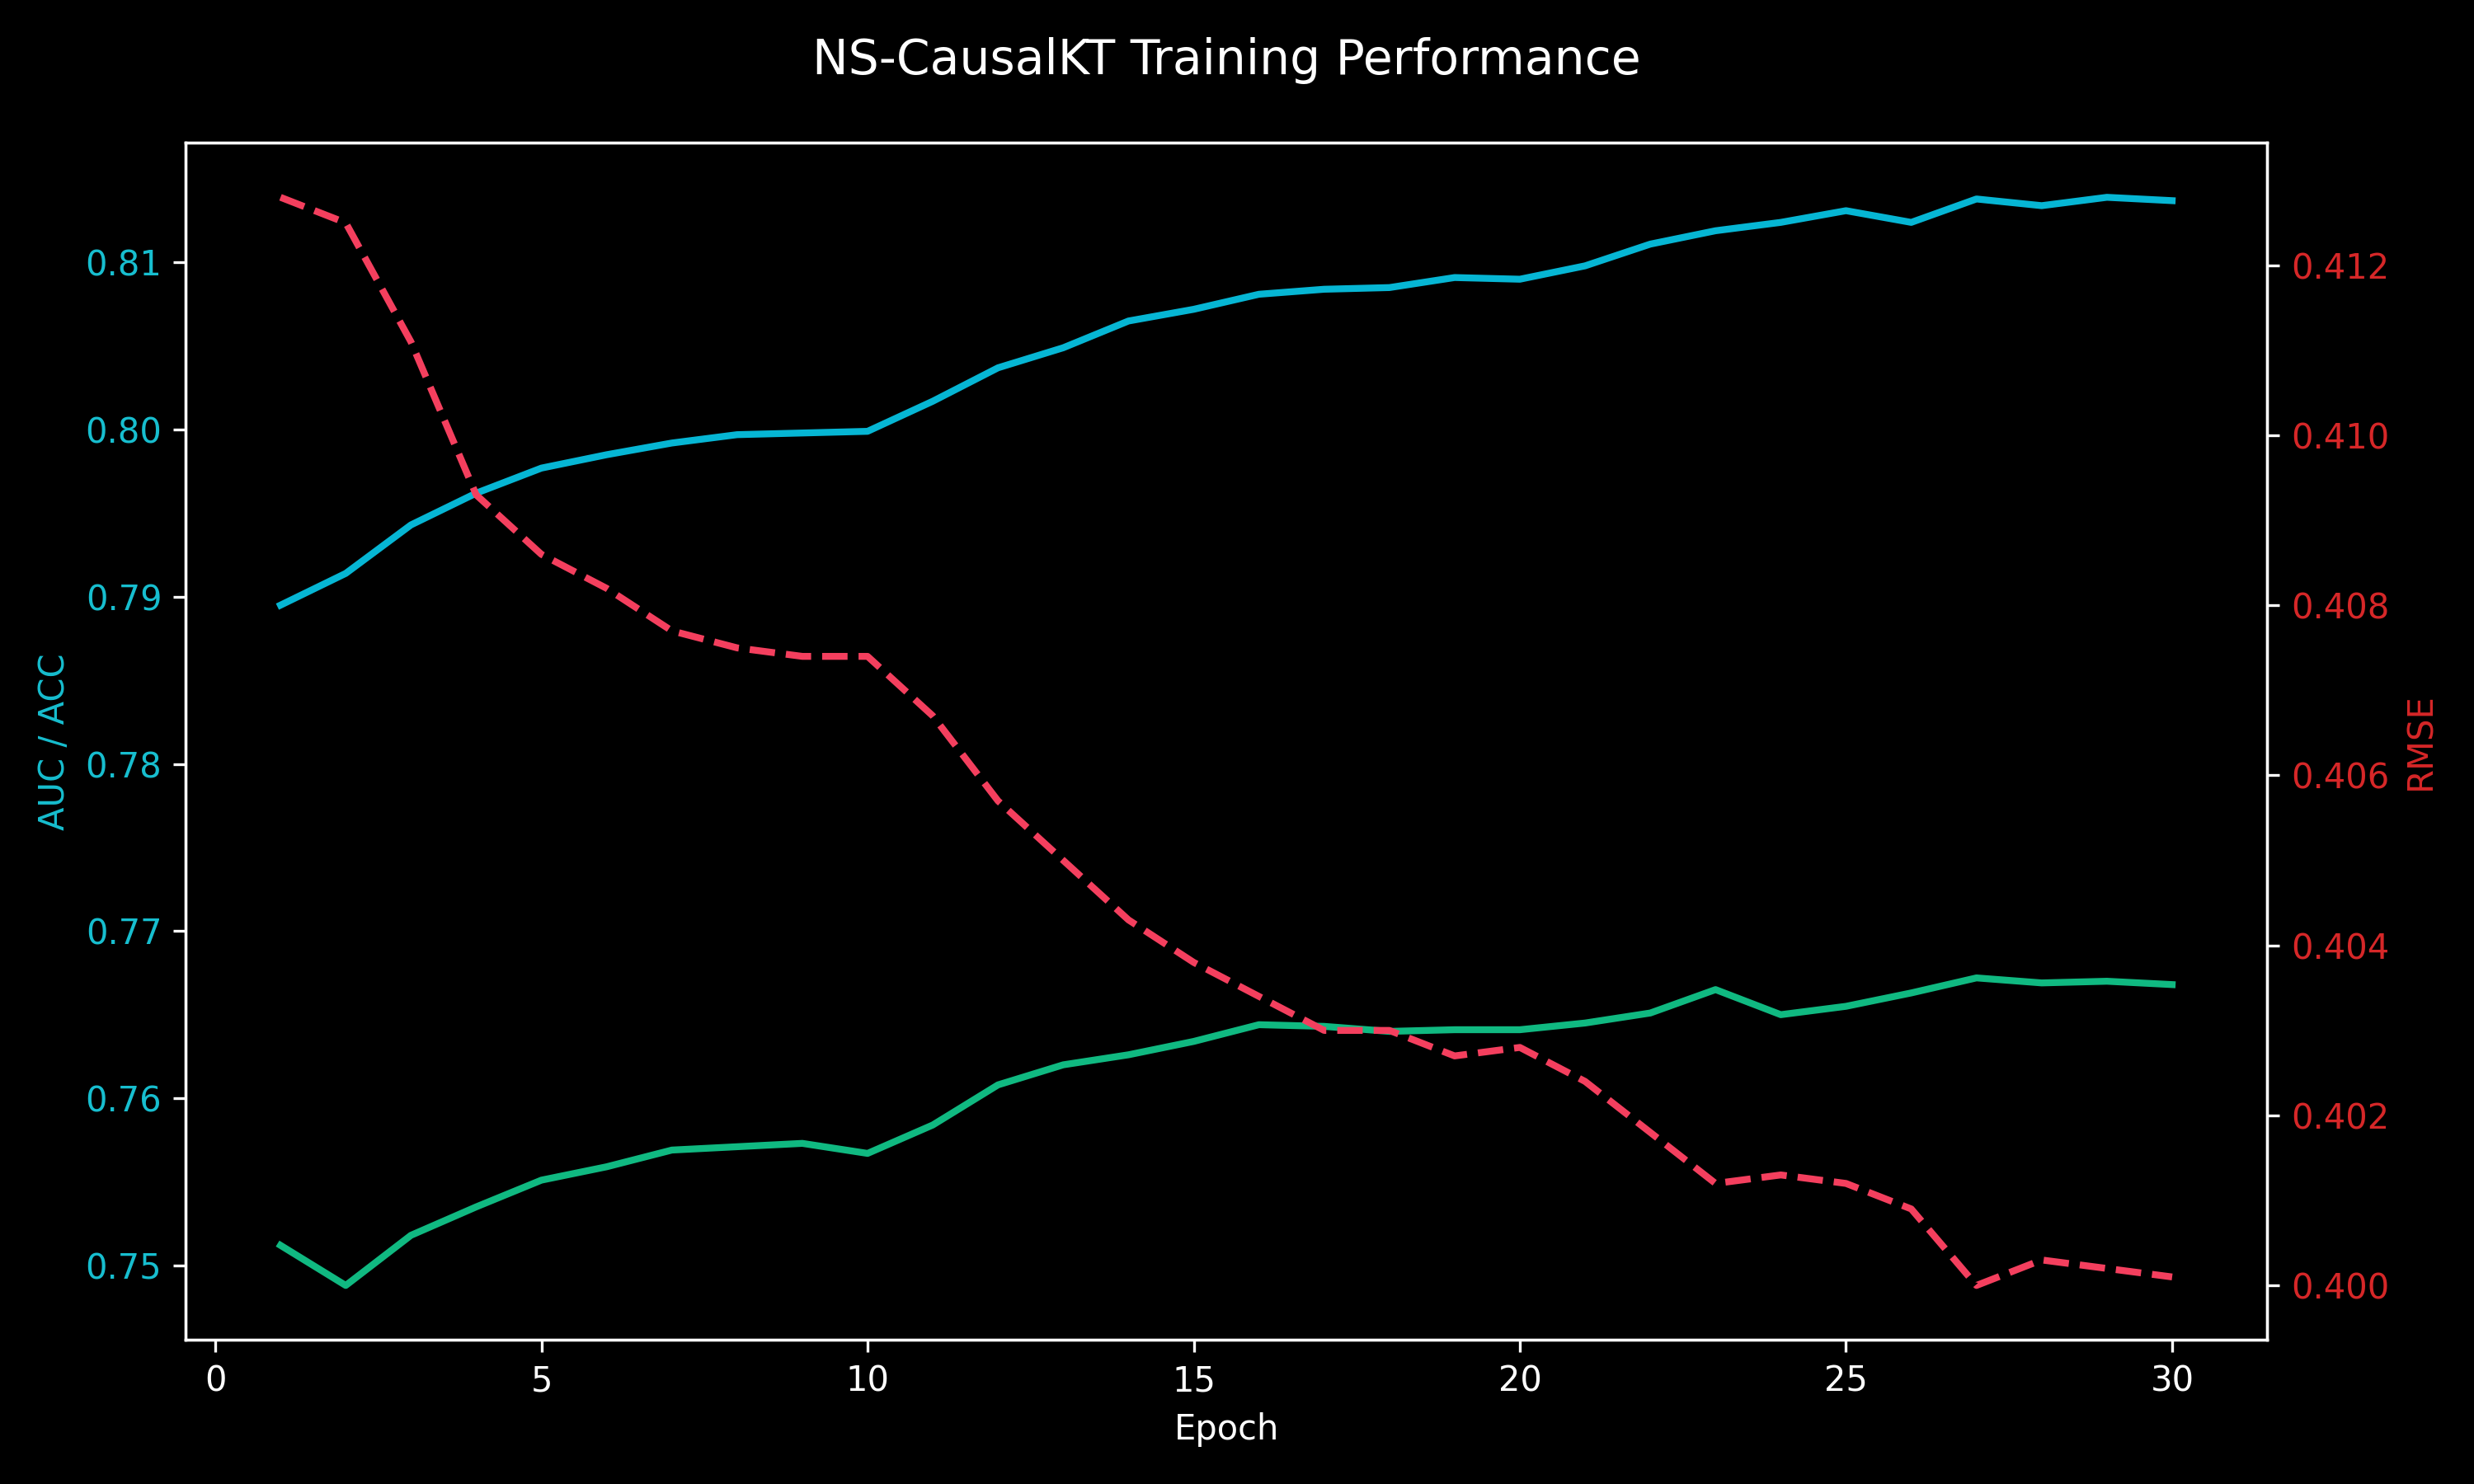
\includegraphics[width=0.8\textwidth]{training_metrics.png}
    \caption{Training metrics over 30 epochs.}
    \label{fig:metrics_ch}
\end{figure}

\section{Causal Analysis}
A key feature of NS-CausalKT is the ability to identify causal effects. Figure \ref{fig:bars_ch} shows a counterfactual analysis for a student struggling with Algebra.

\begin{figure}[h]
    \centering
    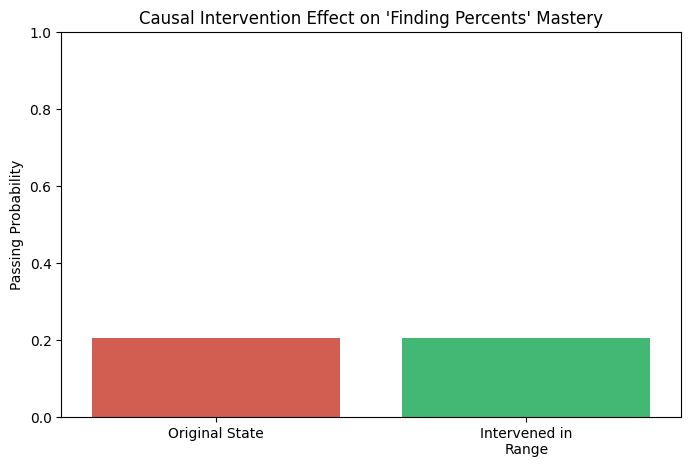
\includegraphics[width=0.6\textwidth]{counterfactual_bars.png}
    \caption{Counterfactual prediction: Simulated score improvement after intervention.}
    \label{fig:bars_ch}
\end{figure}

\section{Visualizing Mastery}
The mastery timeline (Figure \ref{fig:heatmap_ch}) allows educators to see the evolution of a student's knowledge across multiple skills. This provides a granular view that is missing in aggregate scores.

\begin{figure}[h]
    \centering
    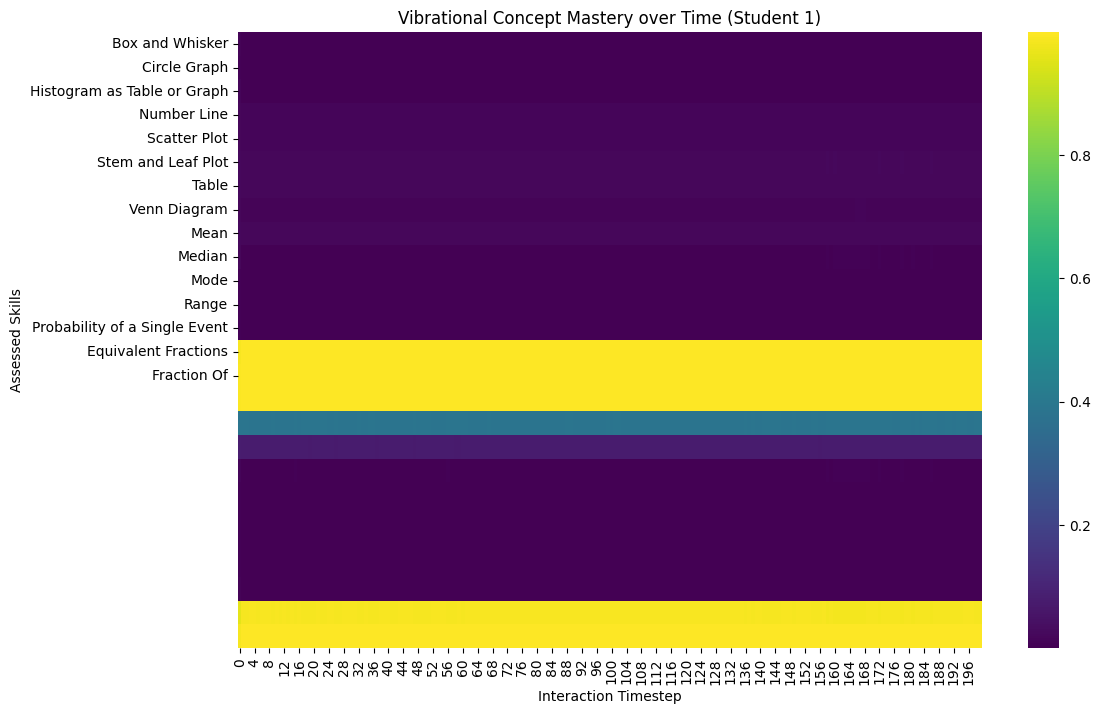
\includegraphics[width=0.8\textwidth]{student_heatmap.png}
    \caption{Student mastery heatmap across different skills.}
    \label{fig:heatmap_ch}
\end{figure}

\section{Discussion}
The results confirm our hypothesis that adding a symbolic layer does not degrade predictive performance but significantly improves interpretability. The model is able to maintain a logically consistent knowledge state, where students are not predicted to master advanced skills if they lack the prerequisites.

\chapter{Technical Specifications}

\section{Project Directory Structure}
The project is organized to separate model logic from the web interface.
\begin{lstlisting}[language=bash]
main el - causal/
├── agentic_ui/           # Frontend (HTML/CSS/JS)
├── backend/              # Local Flask Server
├── models/               # PyTorch Model Definitions (NS-CausalKT, DKT, AKT)
├── checkpoints/          # Trained weights and logs
├── data/                 # ASSISTments dataset
├── report/               # This documentation and assets
└── train.py/eval.py      # Core scripts
\end{lstlisting}

\section{Dependency List}
The following Python packages are required to run the full pipeline:
\begin{itemize}
    \item \texttt{torch >= 2.3.0}: Deep learning framework.
    \item \texttt{torch-geometric}: Graph Convolutional Network support.
    \item \texttt{flask}: Web backend.
    \item \texttt{openai}: Multimodal agent integration.
    \item \texttt{pandas / numpy}: Data manipulation.
    \item \texttt{matplotlib / seaborn}: Causal visualization generation.
\end{itemize}

\section{Hardware Requirements}
For optimal training performance, the following hardware is recommended:
\begin{itemize}
    \item **GPU**: NVIDIA GeForce RTX 3060 or higher (8GB VRAM).
    \item **RAM**: 16GB.
    \item **Storage**: 2GB for dataset and checkpoints.
\end{itemize}

\chapter{Conclusion \& Future Work}

\section{Summary}
In this project, we developed **NS-CausalKT**, a Neuro-Symbolic Causal Knowledge Tracing framework. We successfully integrated deep learning with symbolic logic and causal reasoning to create a model that is both accurate and interpretable. Our system provides:
\begin{itemize}
    \item **Explainable Diagnostics**: Identifying root causes of failure through ACE rankings.
    \item **Interactive Simulations**: Simulating pedagogical interventions through do-calculus.
    \item **Agentic Feedback**: Automated grading of handwritten work with diagnostic depth.
\end{itemize}

\section{Limitations}
While NS-CausalKT shows promising results, it has some limitations:
\begin{itemize}
    \item **Computational Cost**: The joint training of three layers is more computationally intensive than pure DKT.
    \item **Prerequisite Dependency**: The model relies on a high-quality prerequisite graph. If the graph contains errors, the symbolic layer may enforce incorrect mastery patterns.
\end{itemize}

\section{Future Work}
Future research could explore:
\begin{itemize}
    \item **Dynamic Graph Learning**: Automatically learning the prerequisite graph from raw data instead of relying on domain experts.
    \item **Multimodal Knowledge Tracing**: Integrating student's facial expressions or gaze data to further refine the knowledge state estimate.
    \item **Reinforcement Learning (RL)**: Using the causal engine as a reward function for an RL agent to generate optimal learning paths.
\end{itemize}

\section{Personal Reflections}
This project has been a valuable learning experience in building a complex, integrated AI system. Handling challenges like API authentication, dataset preprocessing, and neuro-symbolic integration has provided deep insights into the future of trustworthy and interpretable Artificial Intelligence.


\bibliographystyle{plain}
\begin{thebibliography}{99}
\bibitem{dkt} Piech, C., Bassen, J., Huang, J., Ganguli, S., Sahami, M., Guibas, L. J., \& Sohl-Dickstein, J. (2015). Deep knowledge tracing. Advances in neural information processing systems, 28.
\bibitem{akt} Ghosh, A., Heffernan, N., \& Lan, A. S. (2020). Context-aware attentive knowledge tracing. In Proceedings of the 26th ACM SIGKDD international conference on knowledge discovery \& data mining.
\bibitem{pearl} Pearl, J. (2009). Causality. Cambridge university press.
\bibitem{ltn} Serafini, L., \& Garcez, A. D. (2016). Logic tensor networks: Deep learning and logical reasoning from data and knowledge. arXiv preprint arXiv:1606.04422.
\end{thebibliography}

\end{document}
